\section{Sistema de Intercambio de Gases}
%
El sistema de intercambio de gases es el objeto de este trabajo, se ocupa de
los procesos de admisión y escape que consisten en admitir una carga de mezcla
fresca y expulsar los gases quemados al final de cada ciclo.
%
La masa de aire inductada limita la cantidad de combustible que se puede
quemar, del mismo modo que la cantidad de gases quemados que se pueden extraer
al final de cada ciclo limita la cantidad de masa fresca que puede ingresar a
la cámara de combustión.
%
Por estos motivos es importante que la geometría de este sistema permita que
estos procesos se realicen de manera eficiente, maximizando la cantidad de
mezcla disponible para la combustión en cada ciclo.
%
Otros objetivos de este sistema son el de preparar la mezcla~\footnote{En el
caso de motores SI que admiten mezclas de aire y combustible} y brindar un
flujo que favorezca el proceso de combustión.


El MRCVC no posee válvulas que definan el inicio y fin de los procesos de
admisión y escape, sino que posee puertos similares a lumbreras.
%
Esto significa que sin un mecanismo adicional, la posición y geometría de los
mismos define el inicio y fin de estos procesos.
%
La diferencia en geometría entre un motor con válvulas y uno sin, se puede
observar en la Figura~\ref{fig:puerto_valvula}, en la que se ve un corte
transversal de un puerto de admisión de un motor alternativo convencional y
puertos de admisión/escape en el estator de un motor Wankel.

\begin{figure}
  \centering
    \subfloat[][Puerto con Válvulas\parencite{2carpros}]{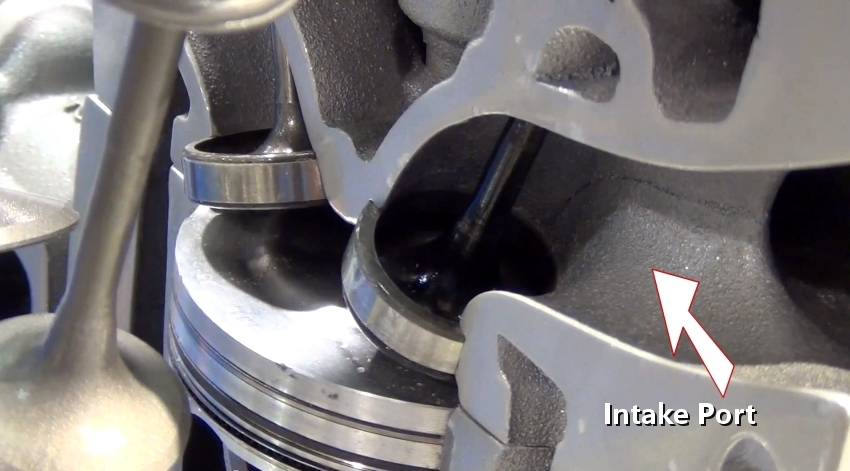
\includegraphics[width=0.5\textwidth]{ports_cut.png}}
    \subfloat[][Lumbrera\protect\footnotemark]{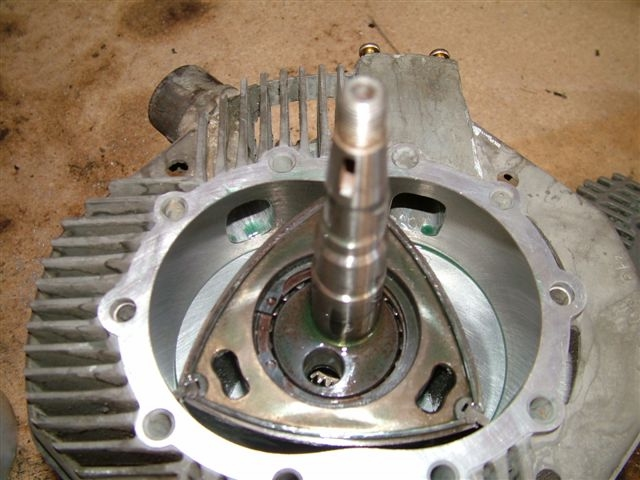
\includegraphics[width=0.5\textwidth]{puertos_rotativo.png}}
  \caption{Diferentes sistemas de intercambio de gases}\label{fig:puerto_valvula}
\end{figure}

\footnotetext{\url{https://www.rx7club.com/old-school-other-rotary-63/latest-project-periphial-port-motorbike-746910/}}

En este trabajo se utilizó un sistema simplificado, que consta de un tubo de
diámetro $D$ y longitud $L$ tanto para la admisión como para el escape
(Fig.~\ref{fig:croquis_mrcvc}).

% NOTA: aca podria poner una comparativa de rendimientos volumetricos, potencia y
% torque para un motor con puertos con mayor y menor apertura, mayor y menor
% diametro

\begin{figure}
    \centering
    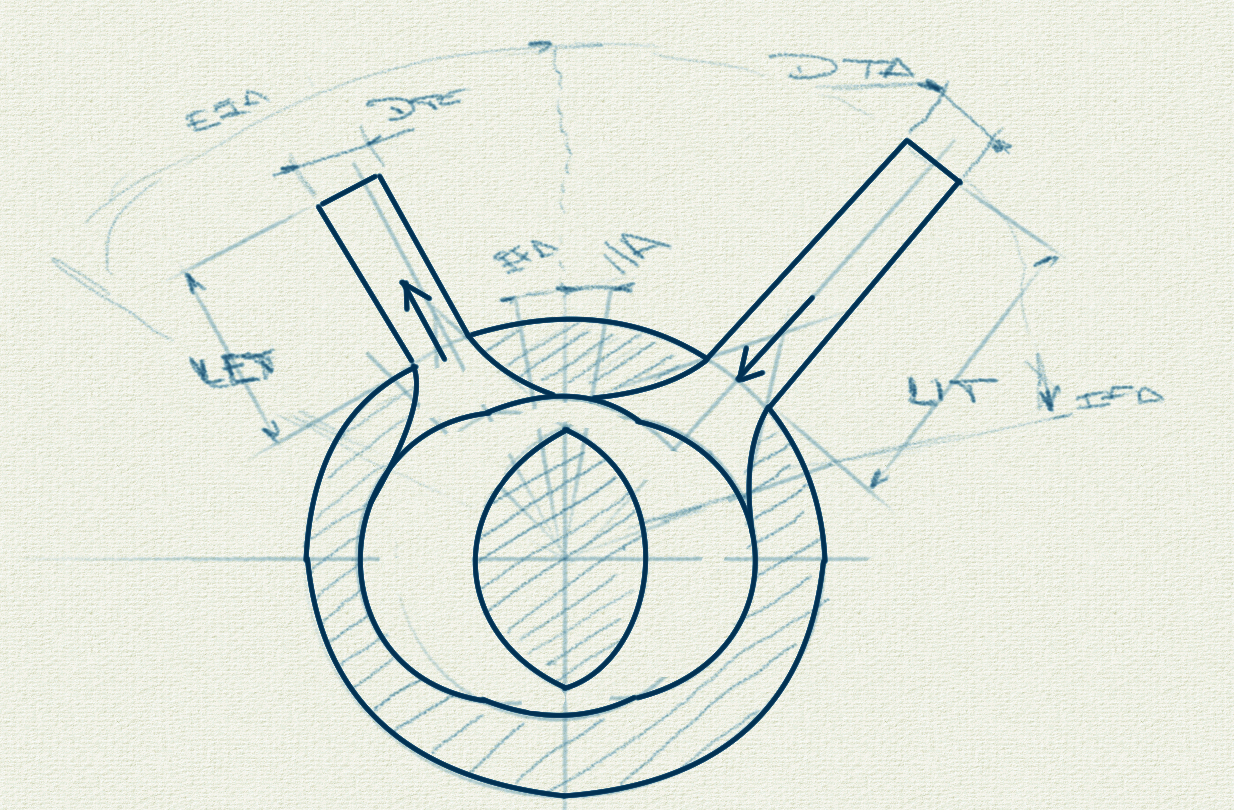
\includegraphics[width=0.5\textwidth]{croquis_motor.png}
    \caption{Sistema de Intercambio de gases simplificado}\label{fig:croquis_mrcvc}
\end{figure}

En trabajos anteriores~\parencite{mrcvc_geom} se determinó que los puertos
ubicados sobre el cuerpo central del estator  dan mejores resultados que los
ubicados en la tapa del estator.

\subsection{Indicadores de Rendimiento}\label{sec:indicadores_rendimiento}

Se medirá la eficiencia del sistema de intercambio de gases utilizando el
rendimiento volumétrico $\eta_v$ como principal indicador y la fracción de
gases residuales $x_r$, como indicador secundario.
%
El rendimiento volumétrico se define como la relación entre el caudal
volumétrico de aire que ingresa al sistema de admisión y la velocidad a la que
cambia el volumen dentro de un cilindro.
%

% NOTA: esto lo saco porque ya lo defino con detalle más adelante
\begin{equation}\label{eq:rendVol}
  \eta_v = \frac{2 \dot{m}_a}{\rho_{a,i} V_d N} = \frac{m_a}{\rho_{a,i} V_d}
\end{equation}

Donde $V_D$, es el volumen desplazado, $N$ son las revoluciones por minuto,
$\rho_{a,i}$ en el caso de motores naturalmente aspirados es la densidad del
aire a la entrada del sistema de admisión y $m_a$ es la masa inductada al
cilindro en cada ciclo.

Típicamente, el máximo rendimiento volumétrico encontrado en motores
naturalmente aspirados es de alrededor de $\eta_v = 0.9$.
%
Para poder comparar entre sistemas de admisión de motores naturalmente
aspirados, se suele mantener la densidad de la admisión como la densidad del
aire en condiciones atmosféricas normales (1 atm y 30ºC) 

Por otro lado, la fracción de gases residuales se define como el cociente entre
la masa de gases residuales (son los gases quemados al final de la carrera de
escape), con la masa total atrapada en el cilindro luego del fin de la carrera
de admisión:

\begin{equation}\label{eq:fracRes}
    x_r = \frac{m_r}{m_c} = \frac{m_r}{m_a + m_r} 
\end{equation}

Valores típicos de fracción de gases residuales para motores de combustión
interna rondan el 5\%, estos valores siempre se dan considerando que se está
trabajando a mariposa totalmente abierta.

En algunos motores se utilizan gases de escape para diluir la masa fresca en un
proceso conocido como EGR, con esto se logra controlar las emisiones de $NO_x$,
esta dilución afecta el valor de $x_r$ porque aumenta la cantidad inicial de
masa quemada en cada ciclo.

\begin{equation}\label{eq:fracRes}
    x_r = \frac{m_{EGR} + m_r}{m_c}
\end{equation}

%
% La ubicación angular de los puertos determina la duración de los procesos de
% admisión y escape, además de modificar la forma y el coeficiente de descarga.

% Estos parámetros se ajustan o seleccionan teniendo en cuenta requisitos de
% funcionamiento del motor, por lo que fue necesario establecer una curva de
% rendimiento volumétrico para que la simulación numérica del
% ciclo termodinámico se pueda acoplar al algoritmo de optimización y de este
% modo evaluar los motores contra la curva de rendimiento requerida.
% %
% El criterio de diseño/selección de la curva de $\eta_v$ fué el siguiente:
%
% \begin{itemize}
%   \item que tenga un máximo de rendimiento entre 4000 y 6000 rpm.
%   \item que la curva sea suave
% \end{itemize}
